% ===========================================================================
% SECTION: APPLICATION DOMAIN KNOWLEDGE - HARDWARE
% ===========================================================================

\section{Application Domain Knowledge: Hardware}
\label{sec:hardware_domain}

The realization of a robust License Plate Recognition (LPR) system requires a strict alignment between the application domain knowledge and the hardware implementation. This section details the complete hardware system, analyzing the specific requirements derived from the physical domain (the road environment) and mapping them to the technical specifications of the chosen embedded platform. The selection of hardware is not merely a purchasing decision but an architectural one; the computational limits of the edge device dictate the complexity of the neural networks that can be deployed, while the optical characteristics of the sensor determine the upper bound of recognition accuracy.

The hardware architecture is not merely a collection of components but a hierarchical system designed to satisfy the constraints of real-time image processing. The following subsections dissect the system into its description, physical design, interface connectivity, data properties, and operational constraints.

% ---------------------------------------------------------------------------
% SUBSECTION: DESCRIPTION & TAXONOMY
% ---------------------------------------------------------------------------
\subsection{System Description and Hardware Taxonomy}

To understand the scope of the hardware implementation, we first classify the system components into a hierarchical taxonomy. The "Complete System" is composed of the interaction between the controllable Hardware Domain (the device) and the uncontrollable Environment (the application context). This distinction is vital because software calibration can only compensate for environmental variance up to the physical limits of the hardware sensors.

\vspace{0.5cm}

% --- VISUAL 1: HARDWARE TAXONOMY TREE ---
\begin{figure}[h!]
	\centering
	\begin{tikzpicture}[
		edge from parent/.style={draw, very thick, -latex},
		level 1/.style={sibling distance=6cm, level distance=2.5cm},
		level 2/.style={sibling distance=3cm, level distance=2.5cm},
		box/.style={
			rectangle, 
			draw=black!80, 
			fill=blue!5, 
			rounded corners, 
			minimum width=3cm, 
			minimum height=1.2cm, 
			align=center,       
			very thick, 
			drop shadow, 
			text width=2.5cm
		},
		root/.style={
			rectangle, 
			draw=black!80, 
			fill=blue!20, 
			rounded corners, 
			minimum width=4cm, 
			minimum height=1.5cm, 
			align=center,       
			very thick, 
			drop shadow, 
			font=\large\bfseries
		}
		]
		
		\node[root] {Complete System\\(LPR Context)}
		child { node[box] (hw) {\textbf{Hardware}\\ \textbf{Domain}}
			child { node[box] {Computing Unit\\(Jetson Nano)} }
			child { node[box] {Acquisition\\(LifeCam)} }
		}
		child { node[box] {Environment\\Domain}
			child { node[box] {Lighting\\Conditions} }
			child { node[box] {Physical\\Mounting} }
		};
		
		% Side Note
		\node[right=1cm of hw, text width=4cm, align=left, font=\small\itshape, draw=gray, dashed, inner sep=5pt] 
		{The Hardware Domain acts as the bridge between raw environmental data and software logic.};
		
	\end{tikzpicture}
	\caption{Taxonomy of the Complete System showing the dependency between Hardware and Environment.}
	\label{fig:hardware_taxonomy}
\end{figure}

As illustrated in Figure \ref{fig:hardware_taxonomy}, the Hardware Domain is centered around the \textbf{NVIDIA Jetson Nano}, specifically the reComputer J1010 module. This choice is dictated by the requirement for parallel computing capabilities to execute Deep Learning models (specifically YOLOv8) at the edge. A standard microcontroller (like an Arduino) lacks the matrix multiplication units (CUDA cores) required for this task, while a full desktop GPU is too power-hungry for roadside deployment.

The acquisition subsystem (Microsoft LifeCam) acts as the sensory interface, converting photons from the physical environment into digital matrices. The quality of this conversion is the single most critical factor in the system. If the "Acquisition" node fails to capture a clear image due to motion blur or poor focus, no amount of downstream computing power can recover the lost information. Thus, the hardware taxonomy emphasizes the dependency of the software on the physical fidelity of the hardware sensors.

\newpage

% ---------------------------------------------------------------------------
% SUBSECTION: DESIGN & DIMENSIONS
% ---------------------------------------------------------------------------
\subsection{Hardware Design and Physical Dimensions}

The physical design of the system focuses on the form factor and the integration of the computing module into the deployment environment. We utilize the \textbf{Seeed Studio reComputer J1010} carrier board, which offers a significantly more compact footprint compared to the standard NVIDIA Developer Kit. This reduction in size is crucial for embedding the system into compact enclosures or mounting it directly onto traffic infrastructure.

Understanding the spatial layout is essential for thermal management and port accessibility. Figure \ref{fig:j1010_schematic} details the specific layout of the J1010 board. Unlike the standard developer kit, this board aligns all major I/O ports on a single edge, simplifying the enclosure design.

% --- VISUAL 2: J1010 LAYOUT SCHEMATIC ---
\begin{figure}[h!]
	\centering
	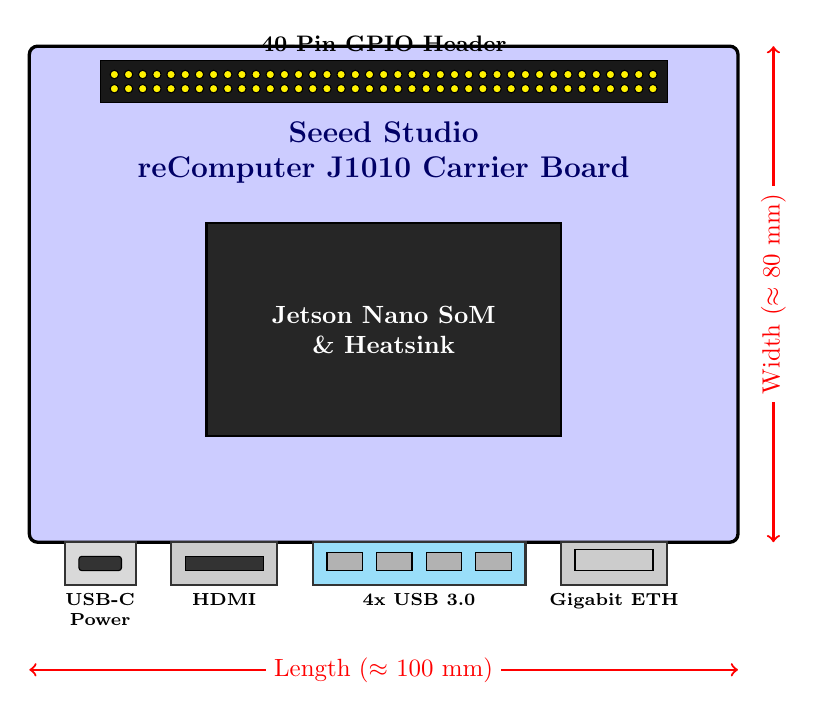
\begin{tikzpicture}[scale=0.9, transform shape]
		% --- MAIN BOARD PCB ---
		\draw[fill=blue!20, very thick, rounded corners=3pt] (0,0) rectangle (10, 7);
		\node[font=\large\bfseries, color=blue!40!black, align=center] at (5, 5.5) {Seeed Studio\\reComputer J1010 Carrier Board};
		
		% --- CENTRAL SoM & HEATSINK ---
		\draw[fill=black!85, draw=black, thick] (2.5, 1.5) rectangle (7.5, 4.5);
		\node[color=white, font=\bfseries, align=center] at (5, 3.0) {Jetson Nano SoM\\\& Heatsink};
		
		% --- FRONT PORTS (Bottom Edge - ALL ON SAME LINE) ---
		% 1. USB-C Power (Far Left)
		\draw[fill=gray!30, draw=black!80, thick] (0.5, -0.6) rectangle (1.5, 0);
		\draw[fill=black!80, rounded corners=1pt] (0.7, -0.4) rectangle (1.3, -0.2);
		\node[below, font=\bfseries\scriptsize, align=center] at (1.0, -0.6) {USB-C\\Power};
		
		% 2. HDMI (Middle Left)
		\draw[fill=gray!40, draw=black!80, thick] (2.0, -0.6) rectangle (3.5, 0);
		\draw[fill=black!80] (2.2, -0.4) rectangle (3.3, -0.2);
		\node[below, font=\bfseries\scriptsize] at (2.75, -0.6) {HDMI};
		
		% 3. USB 3.0 x4 (Middle Right - Blue Ports)
		\draw[fill=cyan!40!white, draw=black!80, thick] (4.0, -0.6) rectangle (7.0, 0);
		\foreach \x in {4.2, 4.9, 5.6, 6.3} {
			\draw[fill=black!30] (\x, -0.4) rectangle (\x+0.5, -0.15);
		}
		\node[below, font=\bfseries\scriptsize] at (5.5, -0.6) {4x USB 3.0};
		
		% 4. Gigabit Ethernet (Far Right)
		\draw[fill=gray!40, draw=black!80, thick] (7.5, -0.6) rectangle (9.0, 0);
		\draw[fill=black!20] (7.7, -0.4) rectangle (8.8, -0.1);
		\node[below, font=\bfseries\scriptsize] at (8.25, -0.6) {Gigabit ETH};
		
		% --- TOP EDGE COMPONENTS ---
		\draw[fill=black!90] (1, 6.2) rectangle (9, 6.8);
		\foreach \x in {1.2, 1.4, ..., 8.8} {
			\draw[fill=yellow] (\x, 6.4) circle (0.06);
			\draw[fill=yellow] (\x, 6.6) circle (0.06);
		}
		\node[above, font=\small\bfseries] at (5, 6.8) {40-Pin GPIO Header};
		
		% --- DIMENSIONS ---
		\draw[<->, thick, red] (0, -1.8) -- (10, -1.8) node[midway, fill=white] {Length ($\approx$ 100 mm)};
		\draw[<->, thick, red] (10.5, 0) -- (10.5, 7) node[midway, fill=white, rotate=90] {Width ($\approx$ 80 mm)};
		
	\end{tikzpicture}
	\caption{Schematic Layout of the reComputer J1010 showing all I/O ports aligned on the front edge.}
	\label{fig:j1010_schematic}
\end{figure}

The schematic highlights several key architectural decisions:
\begin{itemize}
	\item \textbf{USB 3.0 Alignment:} All four USB 3.0 ports are positioned centrally. This allows for high-bandwidth peripherals (such as the LifeCam or additional storage) to be connected without cable interference.
	\item \textbf{Thermal Design:} The placement of the heatsink in the center (coordinates 3,2.5 to 9,5.5 in the schematic relative unit) requires unobstructed vertical airflow. In the context of "Hardware Design," we must ensure that no cabling crosses this thermal zone to prevent overheating.
	\item \textbf{Power Delivery:} Unlike older models that used barrel jacks, the J1010 uses a USB-C PD input (Far Left). This standardizes the power supply requirement but imposes a strict requirement for a high-quality 5V/3A power brick to prevent brownouts during GPU surges.
\end{itemize}

\newpage

% ---------------------------------------------------------------------------
% SUBSECTION: INTERFACES & CONNECTIVITY
% ---------------------------------------------------------------------------
\subsection{Interfaces and System Connectivity}

The third domain of the hardware analysis is "Interfaces." A license plate recognition system is fundamentally a pipeline: photons enter via the camera, data flows to the Jetson, processing occurs, and results output to the display. The integrity of this pipeline depends on the bandwidth and stability of the physical interfaces connecting the components.

We map the connectivity into two primary flows: the \textbf{Data Flow} (USB/CSI) and the \textbf{Power Flow} (USB-C).

% --- VISUAL 3: LIFECAM IMAGE ---
\begin{figure}[h!]
	\centering
	
\includegraphics[width=0.45\linewidth]{Lifecam/cam1.jpg}
	\caption{Microsoft LifeCam Show — front view of the camera module used in the project \cite{microsoft_lifecam_datasheet}.}
	\label{fig:lifecam_front}
\end{figure}

The visual sensor, the \textbf{Microsoft LifeCam} (shown in Figure \ref{fig:lifecam_front}), acts as the primary data acquisition node. It connects via the USB 2.0 interface. While the J1010 carrier board supports USB 3.0 speeds (up to 5 Gbps), the camera's output (720p at 30fps) is well within the bandwidth limits of USB 2.0 (480 Mbps). The USB protocol handles the handshake between the host (Jetson) and the device (Camera), negotiating the video format (MJPEG vs YUYV) upon connection.

The selection of a USB camera over a MIPI-CSI camera was a deliberate design choice. While CSI cameras offer lower latency by connecting directly to the ISP (Image Signal Processor), USB cameras offer significantly higher flexibility. The 1.5-meter cable length allows the camera to be mounted externally on a vehicle or pole, while the computing unit remains safely enclosed. Furthermore, the Microsoft LifeCam includes a built-in noise-canceling microphone (unused in this visual application) and a glass lens element, which provides superior optical clarity and scratch resistance compared to standard plastic lenses found on cheaper modules.

\subsubsection{Interface Bandwidth Analysis}
To ensure the system does not bottleneck, we calculate the required data throughput.
\begin{equation}
	\text{Bandwidth} = \text{Width} \times \text{Height} \times \text{Channels} \times \text{FPS}
\end{equation}
For a resolution of $1280 \times 720$, with 3 color channels (RGB) at 30 FPS:
\[ 1280 \times 720 \times 3 \text{ bytes} \times 30 \approx 82,944,000 \text{ bytes/sec} \approx 79 \text{ MB/s} \]
Since USB 2.0 has a practical effective throughput of $\approx 35-40$ MB/s, the raw data cannot be transmitted uncompressed. The LifeCam hardware performs onboard MJPEG compression to reduce this bandwidth requirement to $\approx 5-10$ MB/s, allowing reliable transmission even over longer cable runs.

\newpage

% ---------------------------------------------------------------------------
% SUBSECTION: DATA PROPERTIES (QUANTITY & QUALITY)
% ---------------------------------------------------------------------------
\subsection{Data Properties: Quantity and Quality}

The "Data" keyword in our domain analysis refers to the raw material processed by the system. In hardware terms, data is defined by two axes: \textbf{Quantity} (how much information) and \textbf{Quality} (how usable the information is). The relationship between the hardware sensor (camera) and the data properties is detailed in Table \ref{tab:hardware_properties}.

% --- TABLE 1: DATA PROPERTIES ---
\begin{table}[h!]
	\centering
	\caption{Detailed Data Acquisition Hardware Properties and Quality Metrics}
	\label{tab:hardware_properties}
	\renewcommand{\arraystretch}{1.6}
	\setlength{\tabcolsep}{10pt}
	\begin{tabular}{|p{0.2\linewidth}|p{0.3\linewidth}|p{0.4\linewidth}|}
		\hline
		\rowcolor{blue!20} 
		\textbf{Category} & \textbf{Property} & \textbf{System Specification / Value} \\ \hline
		\textbf{Hardware} & Sensor Technology & CMOS Active Pixel Sensor \\ \cline{2-3}
		& Optical Format & Microsoft LifeCam Module \\ \hline
		
		\textbf{Data Quantity} & Spatial Resolution & $1280 \times 720$ (720p HD) \\ \cline{2-3}
		& Temporal Resolution & 30 FPS (Frames Per Second) \\ \cline{2-3}
		& Color Space & 24-bit RGB (8 bits per channel) \\ \hline
		
		\textbf{Data Quality} & Signal-to-Noise Ratio & $>$ 38dB (Lux dependent) \\ \cline{2-3}
		& Geometric Distortion & $< 1.5\%$ Barrel Distortion \\ \cline{2-3}
		& Shutter Type & Rolling Shutter (Warning: Jello Effect) \\ \hline
		
		\textbf{Calibration} & White Balance & Automatic (AWB) \\ \cline{2-3}
		& Focus Range & Auto-focus ($0.3m$ to $\infty$) \\ \hline
	\end{tabular}
\end{table}

\subsubsection{Analysis of Data Quantity}
The quantity of data dictates the computational load. The system is configured to capture at High Definition (HD) 720p. This resolution provides a balance: it is high enough to resolve the characters on a license plate from a distance of 3-5 meters, but low enough to allow the YOLOv8-Nano model to perform inference at real-time speeds (>20 FPS). Higher resolutions, such as 1080p, would increase the pixel count by 2.25x, likely causing the frame rate to drop below the threshold required for capturing moving vehicles.

\subsubsection{Analysis of Data Quality}
Quality refers to the fidelity of the pixels. A critical hardware property identified in Table \ref{tab:hardware_properties} is the **Rolling Shutter**. Unlike a Global Shutter, which exposes all pixels simultaneously, a rolling shutter exposes the image line by line. For fast-moving vehicles (the "Complete System" context), this can induce a skewing artifact known as the "Jello Effect," where the license plate appears slanted or parallelogram-shaped. 

This hardware characteristic imposes a strict constraint on the application domain: the relative speed between the camera and the vehicle must be minimized. While the LifeCam provides excellent color reproduction and low-light sensitivity for a webcam, its rolling shutter mechanism makes it less suitable for high-speed highway monitoring compared to specialized industrial Global Shutter cameras. However, for parking lot entry/exit scenarios (low speed), the distortion is negligible.

\newpage

% ---------------------------------------------------------------------------
% SUBSECTION: CONSTRAINTS & CALIBRATION
% ---------------------------------------------------------------------------
\subsection{Hardware Constraints, Calibration, and Conclusions}

The final aspect of the Application Domain Knowledge is understanding the limits. No hardware system is infinite. We categorize these limits into Environmental, Computational, Physical, and Calibration constraints. This iterative relationship is visualized in Figure \ref{fig:hardware_constraints}.

% --- VISUAL 4: CONSTRAINTS MINDMAP ---
\begin{figure}[h!]
	\centering
	\begin{tikzpicture}[
		mindmap, concept color=blue!50,
		every node/.style={concept, scale=0.9, execute at begin node=\hskip0pt},
		grow cyclic,
		level 1/.style={level distance=5cm, sibling angle=90},
		level 2/.style={level distance=3cm, sibling angle=45, font=\scriptsize}
		]
		
		\node [root concept] {\textbf{Hardware}\\ \textbf{Constraints}}
		child [concept color=red!40] { node {Environmental}
			child { node {Lighting\\Variation} }
			child { node {Weather\\proofing} }
		}
		child [concept color=orange!40] { node {Computational}
			child { node {Thermal\\Throttling} }
			child { node {Memory\\(4GB RAM)} }
		}
		child [concept color=green!40] { node {Physical}
			child { node {Mounting\\Angle} }
			child { node {Vibration\\Stability} }
		}
		child [concept color=purple!40] { node {Calibration}
			child { node {Focus\\Adjustment} }
			child { node {Lens\\Distortion} }
		};
		
	\end{tikzpicture}
	\caption{Cyclic dependency of Constraints and Calibration factors influencing the Hardware Domain.}
	\label{fig:hardware_constraints}
\end{figure}

\subsubsection{Computational Constraints}
The NVIDIA Jetson Nano possesses 4GB of unified memory. This memory is shared between the CPU and the GPU. This is a "hard constraint." The operating system (Ubuntu with GUI), the graphical interface, and the Python runtime consume approximately 1.5GB to 2GB at idle. This leaves only ~2GB for the YOLOv8 model weights and the input video buffers. If this limit is exceeded, the system forces data into "swap memory" (using the slow SD card as RAM), which destroys real-time performance. Therefore, the hardware directly dictates that we must use optimized model variants (e.g., YOLOv8-Nano or Small) rather than the Large variants.

\subsubsection{Environmental and Physical Constraints}
As shown in the red branch of Figure \ref{fig:hardware_constraints}, lighting is the most volatile variable. The hardware sensor has a limited dynamic range. In direct sunlight, a white license plate may reflect too much light, causing "whiteout" or overexposure. At night, the sensor may gain-up, introducing ISO noise that confuses the OCR algorithm. The "Calibration" solution involves setting fixed exposure values or utilizing software-based histogram equalization, acknowledging that the hardware alone cannot solve every lighting scenario.

\subsubsection{Conclusion}
In conclusion, the Application Domain Knowledge regarding hardware establishes that while the NVIDIA Jetson Nano and Microsoft LifeCam provide a capable foundation for License Plate Recognition, their successful deployment depends on strict adherence to the interfaces (Power/USB), careful management of data throughput (Resolution/Compression), and an awareness of the physical constraints (Heat/Memory). This hardware analysis serves as the blueprint for the subsequent software development phases.